\documentclass[a4paper, 14pt,russian]{extarticle}

\usepackage[russian]{babel}
\usepackage[T2A]{fontenc}
\usepackage[utf8]{inputenc}
%Соответствующий математический шрифт для Times new roman
\usepackage{newtxmath}
\usepackage{fontspec} 
\usepackage{multirow}
%\usepackage{polyglossia}
%Times new roman
\defaultfontfeatures{Ligatures={TeX},Renderer=Basic} 
\setmainfont[Ligatures={TeX,Historic}]{Times New Roman}
\setmainfont{Times New Roman}
\setsansfont{Arial}
\setmonofont{Courier New}
\newfontfamily\cyrillicfont[Script=Cyrillic]{Times New Roman}
\newfontfamily\cyrillicfontsf[Script=Cyrillic]{Arial}
\newfontfamily\cyrillicfonttt[Script=Cyrillic]{Courier New}

%\setdefaultlanguage{russian}

%Геометрия
\usepackage{geometry}
\geometry{top=20mm}
\geometry{bottom=15mm}
\geometry{left=20mm}
\geometry{right=15mm}
\usepackage{setspace}
%Нормальные дроби через запятую
\usepackage{ncccomma}

\newcommand{\changefont}{%
	\fontsize{12}{11}\selectfont
}

%Заголовки
\usepackage{fancyhdr}
\pagestyle{fancy}
\fancyhf{}
%\renewcommand{\sectionmark}[1]{\markright{#1}}
\fancyhead[R]{\changefont \slshape \leftmark}
\fancyhead[L]{\changefont \slshape \rightmark}
%\newcommand{\ssubsection}[1]{\subsection*{#1}
%	\addcontentsline{toc}{subsection}{#1}
%	\markright{#1}{}}
\cfoot{\thepage}

%\полуторный интервал
\setstretch{1.15}
\setlength{\parindent}{1.25cm}

\usepackage{amsmath, amsfonts, mathtools}
\usepackage{physics}
\usepackage{indentfirst}
\usepackage{xcolor}
\usepackage{alltt}
\usepackage{graphicx}
\usepackage{wrapfig}
\usepackage{pgfplots}

%Настройка ссылок
\usepackage{hyperref}
%\usepackage{upgreek}
%\renewcommand{\beta}{\upbeta}
\hypersetup{
	colorlinks,
	citecolor=black,
	filecolor=black,
	linkcolor=black,
	urlcolor=black
}
\usepackage{caption}
\DeclareCaptionLabelSeparator{dot}{. }
\captionsetup{justification=centering,labelsep=dot}
\usepackage{titlesec}

%Формат заголовков
\titleformat{\section}{\bfseries\filcenter\Large}{\thesection}{1em}{}
\titleformat{\subsection}{\bfseries\filcenter\large}{\thesubsection}{1em}{}
\titleformat{\subsubsection}{\bfseries\filcenter\normalsize}{\thesubsubsection}{1em}{}

\usepackage{chngcntr}

%Включить в нумерацию картинок раздел
\counterwithin{figure}{section}

%Листинги кода и их стили
\usepackage{listings}
\usepackage{minted}
\lstdefinestyle{c++} {
	language=C++,
	breaklines=true,
	frame=single,
	numbers=left,
	basicstyle=\footnotesize\ttfamily,
	keywordstyle=\bfseries\color{green!40!black},
	commentstyle=\itshape\color{purple!40!black},
	identifierstyle=\color{blue},
	backgroundcolor=\color{gray!10!white},
}

\lstdefinestyle{python}{
	language=Python,
	breaklines=true,
	frame=single,
	numbers=left,
	keywordstyle=\bfseries\color{green!40!black},
	frame=lines,
	basicstyle=\footnotesize\rmfamily
}

\lstdefinestyle{cmd}{
	breaklines=true,
	frame=single,
	basicstyle=\footnotesize\ttfamily,
	frame=lines
	basicstyle=\footnotesize
}
\usepackage{tikz}
\usepackage{tkz-base}
\usetikzlibrary{quotes,angles}
\usetikzlibrary {arrows.meta}
%\usepackage{tkz-euclide}
\usetikzlibrary{calc}
\usetikzlibrary{shapes.geometric, shapes.misc, arrows}

\tikzstyle{startstop} = [rectangle, rounded corners, 
minimum width=3cm, 
minimum height=1cm,
text centered, 
draw=black]

\tikzstyle{io} = [trapezium, 
trapezium stretches=true, % A later addition
trapezium left angle=70, 
trapezium right angle=110, 
minimum width=3cm, 
minimum height=1cm, text centered, 
draw=black]

\tikzstyle{process} = [rectangle, 
minimum width=3cm, 
minimum height=1cm, 
text centered, 
text width=5cm, 
draw=black]

\tikzstyle{decision} = [diamond, 
minimum width=3cm, 
minimum height=1cm, 
text centered, 
draw=black]
\tikzstyle{arrow} = [thick,->,>=stealth]

\tikzstyle{startfor} = [chamfered rectangle, 
chamfered rectangle corners={north west, north east},
minimum width=3cm, 
minimum height=1cm, 
text centered, 
draw=black]

\tikzstyle{endfor} = [chamfered rectangle, 
chamfered rectangle corners={south west, south east},
minimum width=3cm, 
minimum height=1cm, 
text centered, 
draw=black]
\tikzstyle{arrow} = [thick,->,>=stealth]

\begin{document}
	
	\begin{titlepage}
	\newpage
	\begin{center}
		
\includegraphics[width=\textwidth]{png/tit.png}
		Институт информационных и вычислительных технологий \\
		Кафедра управления и интеллектуальных технологий
		\vspace{1.25cm}
	\end{center}
	
	\vspace{1.2em}
	
	\begin{center}
		%\textsc{\textbf{}}
		\begin{spacing}{1}
			{\Large Лабораторная работа №2\linebreak
				По дисциплине <<Теория автоматического управления>> \\}
			\large{\bf<<Анализ динамики нелинейных систем методом фазовой плоскости>>}
		\end{spacing}
	\end{center}
	
	\vspace{5em}
	
	
	\vspace{6em}
	
	\noindent Выполнили студенты: Михайловский М., Томчук В. \\
	Группа: А-03-21 \\
	Бригада: 1\\
	Проверил: Деменьтьев В.\,Ю.
	
	
	\vspace{\fill}
	
	\begin{center}
		Москва 2024
	\end{center}
	
\end{titlepage}
	\pagenumbering{arabic}
	\setcounter{page}{2}
	\tableofcontents
	\newpage
	
	\newcommand{\diag}[1]{\mathrm{diag}\,#1}
	\renewcommand{\sp}[1]{\mathrm{sp}\,#1}

	\section{Подготовка к работе}
	\subsection{Передаточные функции системы}
	
	Дана импульсная система автоматического управления (ИСАУ) с периодом квантования импульсного элемента $T$, представленная на рис. \ref{ss}. 

	\begin{center}
		\begin{tikzpicture}
			% Sum shape
			\drawsum{sum}{(0,0)};
			\fillsumsouth{sum};
			\draw [arrow] ($ (sum) + (-2cm,0) $) -- (sum) node[midway, above] {$g(t)$};
			\drawIIE{IIE}{($ (sum.east) + (2cm, 0) $)};
			
			\node (form) [block, right=2.5cm] at (IIE) {$W_\text{ф}(p)$};   
			\node (nepr) [block, right=2.5cm] at (form) {$W_\text{н}(p)$};   
			
			\draw [arrow] (sum) -- (IIE) node [midway,above]{$x(t)$};
			\draw [arrow] (IIE) -- (form) node [midway,above]{$x^{*}(t)$};
			\draw [arrow] (form) -- (nepr) node [midway,above]{$x^{*}_\text{ф}(t)$};
			\draw[arrow] (nepr.east) -- ++ (1.25cm,0) node [midway](output){}node[midway,above]{$y(t)$};
			\draw[arrow]  (output.center) |- ($ (form) + (0, -1.5cm) $) -| (sum.south);
		\end{tikzpicture}
		\begin{equation*}
			W_\text{ф}(p) = 1,\; W_\text{н}(p) = \frac{k_1 k_2}{p(1+T_1 p)}, \text{ где } k_1 = 2,\, k_2 = 1,\, T_1 = 0,1,\, T = 0,3
			\label{system_pars}
		\end{equation*}
		\vspace{-0.75cm}
		\captionof{figure}{Структурная схема импульсной системы автоматического управления}
		\label{ss}
	\end{center}

	Передаточная функция разомкнутой системы будет иметь вид (\ref{w_raz}):
	\begin{multline}
		W^*_\text{р} (p) = \overline{D}[W_\text{ф}(p) \cdot W_\text{н}(p)] = k_1 k_2 \overline{D} \left[\frac{1}{p(1+pT_1)}\right] = \\ = k_1 k_2 \overline{D} \left[ \frac{1}{p} - \frac{T_1}{1+T_1 p} \right] = k_1 k_2 \left[ \frac{e^{pT}}{e^{pT} - 1} - \frac{e^{pT}}{e^{pT} - e^{-\frac{T}{T_1}}} \right] = \\ =
		\frac{k_1 k_2 \left(1- e^{-\frac{T}{T_1}}\right) e^{pT}}{e^{2pT} - \left(1 + e^{-\frac{T}{T_1}}\right)e^{pT} + e^{-\frac{T}{T_1}}} = \frac{1,9 e^{pT}}{e^{2pT} - 1,05 e^{pT} + 0,05}.
		\label{w_raz}
	\end{multline}

	С помощью $W^*_\text{р}(p)$ найдем передаточную функцию замкнутой системы:
	\begin{multline}
		W^*_\text{з}(p) = \frac{W^*_\text{р} (p)}{1 + W^*_\text{р} (p)} = \frac{k_1 k_2 \left(1- e^{-\frac{T}{T_1}}\right) e^{pT}}
		{k_1 k_2\left(1- e^{-\frac{T}{T_1}}\right)e^{pT} 
			+ \left( e^{2pT} - \left(1 + e^{-\frac{T}{T_1}}\right)e^{pT} + e^{-\frac{T}{T_1}} \right)} = \\ 
		= \frac{k_1 k_2 \left(1- e^{-\frac{T}{T_1}}\right) e^{pT}}
		{e^{2pT} + \left( 1 + e^{-\frac{T}{T_1}} \right) \left( k_1 k_2 \cdot \th{\frac{T}{2T_1}} - 1 \right) e^{pT} + e^{-\frac{T}{T_1}}} = \frac{1,9 e^{pT}}{e^{2pT} + 0,85 e^{pT} + 0,05 }.
		\label{w_zam}
	\end{multline}
	
	\subsection{Устойчивость замкнутой системы}
	
	Проверим устойчивость системы по критерию Гурвица. Характеристическое уравнение (ХУ) замкнутой системы:
	\begin{equation*}
		C^* (p) = e^{2pT} + \left( 1 + e^{-\frac{T}{T_1}} \right) \left( k_1 k_2 \cdot \th{\frac{T}{2T_1}} - 1 \right) e^{pT} + e^{-\frac{T}{T_1}} = e^{2pT} + a_1 e^{pT} + a_2.
	\end{equation*}
	
	Переходя к изображениям $Z$-преобразования и вводя билинейное преобразование $\left( e^{pT} = z = \dfrac{1+V}{1-V}\right)$, получим ХУ непрерывной системы (\ref{k_sys}), соответствующее исследуемой замкнутой ИСАУ, которая является устойчивой или неустойчивой одновременно с исследуемой системой, описанной на рис. \ref{ss}:
	\begin{multline}
		\left(\frac{1+V}{1-V}\right)^2 + a_1 \left(\frac{1+V}{1-V}\right) + a_2 = 0 \Rightarrow (1+V)^2 + a_1 (1 - V^2) + a_2 (1 - V)^2 = 0 \Leftrightarrow \\ 
		\Leftrightarrow (1 - a_1 + a_2)V^2 + 2(1 - a_2)V + 1 + a_1 + a_2 = 0
		\label{k_sys}
	\end{multline}

	По критерию Гурвица для непрерывных систем 2-го порядка, система, соответствующая ХУ (\ref{k_sys}) будет устойчивой тогда и только тогда, когда все коэффициенты данного многочлена относительно $V$ будут одного знака:
	\begin{equation}
		\begin{cases}
			1 + a_1 + a_2 = k_1 k_2 \left( 1 + e^{-\frac{T}{T_1}} \right) \th{\frac{T}{2T_1}} > 0, &\forall k_1 \cdot k_2\in (0,\;+\infty) \\
			1 - a_2 = 1 - e^{-\frac{T}{T_1}} > 0, &\forall k_1 \cdot  k_2\in[0,\;+\infty) \\
			1 - a_1 + a_2 = \left( 1 + e^{-\frac{T}{T_1}} \right) \left(2 - k_1 k_2 \th{\frac{T}{2T_1}} \right) > 0, &\forall k_1\cdot k_2 \in \left[0,\;2\cth{\frac{T}{2T_1}}\right) 			 	
		\end{cases}
		\label{ust_eq}
	\end{equation}

	Отсюда, очевидно, граничный коэффициент усиления $k_\text{гр} = 2 \cth{\frac{T}{2T_1}} = 2,21$. 
	
	\section{Выполнение работы}
	
	Для рассматриваемой системы были заданы параметры, представленные на рис. \ref{input}. Как видим рассчитанная передаточная функция разомкнутой системы совпала с полученной в подготовке (\ref{w_raz})
	
	\begin{center}
		\noindent \begin{minipage}{.45\textwidth}
			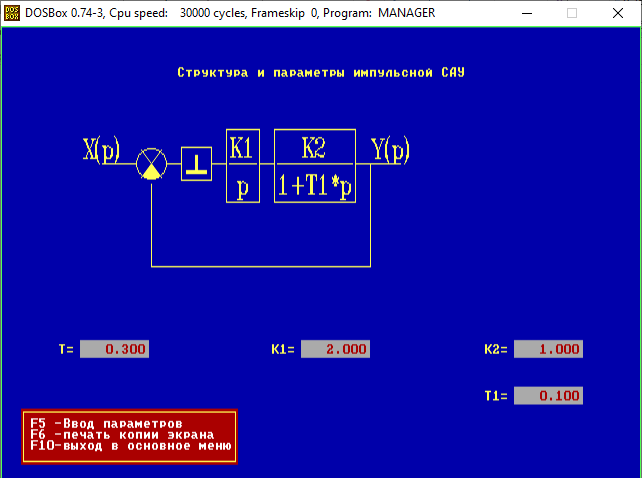
\includegraphics[width=\textwidth]{png/scheme.png}
		\end{minipage} \begin{minipage}{.45\textwidth}
		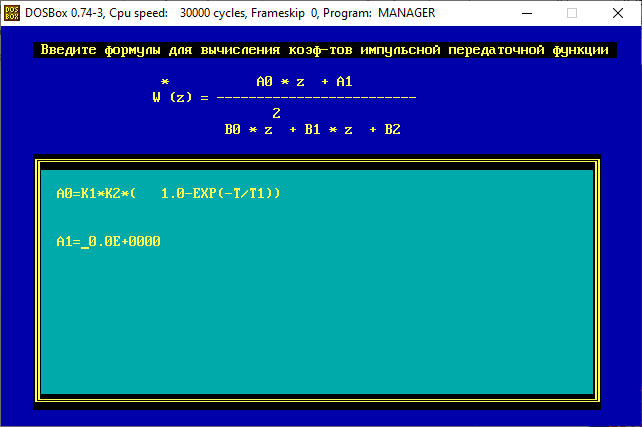
\includegraphics[width=\textwidth]{png/pars1.png}
		\end{minipage}
		\begin{minipage}{.45\textwidth}
			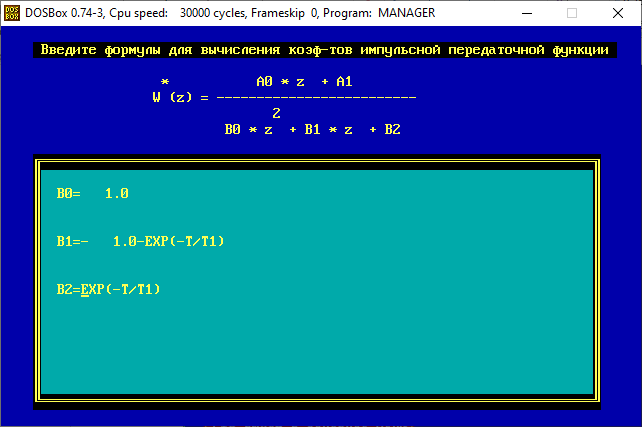
\includegraphics[width=\textwidth]{png/pars2.png}
		\end{minipage} \begin{minipage}{.45\textwidth}
			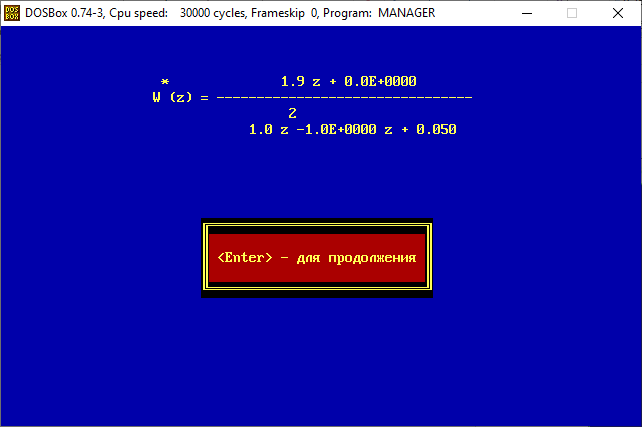
\includegraphics[width=\textwidth]{png/w(z).png}
		\end{minipage}
		\captionof{figure}{Введенные параметры системы в лабораторной программе}
		\label{input}
	\end{center}
	
	\subsection{Рассмотрение ИСАУ как САУ}
	
	Сравнение переходных процессов в изначальной системе с непрерывной системе приведено на рис. \ref{tipoSau1}.
	
	\begin{figure}[h]
		\centering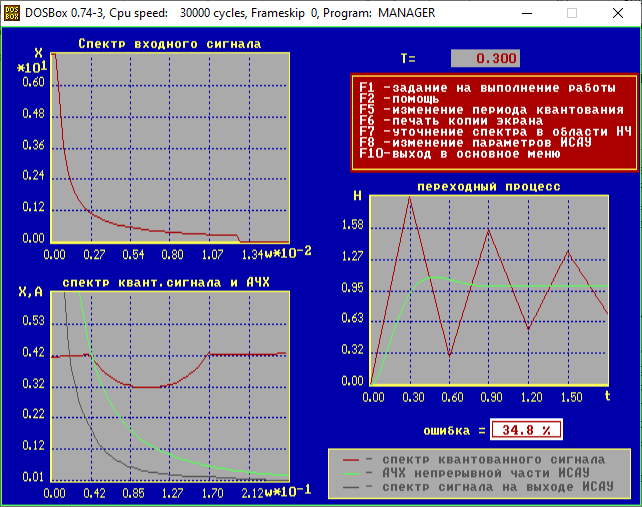
\includegraphics[width=.6\textwidth]{png/graph1.png}
		\caption{Сравнение переходных процессов в САУ и ИСАУ}
		\label{tipoSau1}
	\end{figure}
	
	Как видно из рисунка, процессы плохо совпадают, по характеру и полученным значениям. Рассматривая спектральные характеристики, можно отметить, что спектр квантованного сигнала $\left|Y^* (j\omega)\right|$ не похож на АЧХ непрерывной части $\left|Y(j\omega)\right|$.
	
	\begin{center}
		\noindent \begin{minipage}{.45\textwidth}
			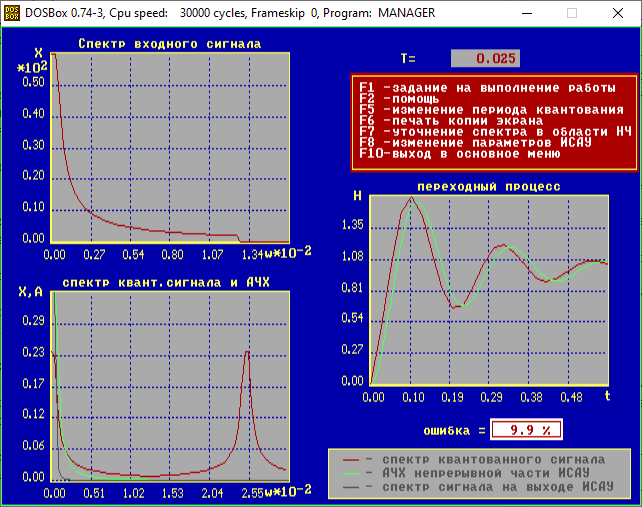
\includegraphics[width=\textwidth]{png/graph2.png}
			\centering{а)}
		\end{minipage} \begin{minipage}{.45\textwidth}
			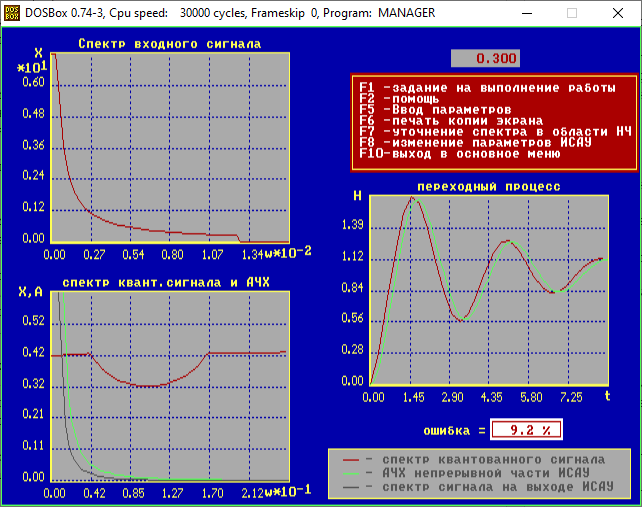
\includegraphics[width=\textwidth]{png/graph3.png}
			\centering{б)}
		\end{minipage}
		\captionof{figure}{ИСАУ, которые можно рассматривать как САУ: а) коррекция $T=0,025$ с, б) коррекция $T_1 = 2$ с}
		\label{tipoSauFig}
	\end{center}

	Если же $\left|Y^* (j\omega)\right| \approx \left|Y(j\omega)\right|$ то ИСАУ, можно рассматривать как САУ (рис. \ref{tipoSauFig}). Это имеет место, если $\omega_0 = \frac{2 \pi}{T} \geqslant \omega_\text{с} + \omega_\text{гр}$, где $\omega_\text{с}$ -- частота среза АЧХ непрерывной части, $\omega_\text{гр}$ -- частота, начиная с которой финитный спектр входного сигнала практически равен нулю $\left|X(j(\omega_\text{гр} + \alpha))\right| \approx 0,\;\forall \alpha\geqslant 0$. 
	
	В нашем случае можно по графикам принять $\omega_\text{гр} = 50\,\text{с}^{-1}$ и $\omega_\text{с} = 10\,\text{с}^{-1}$. Видно, что на рис. \ref{tipoSau1} $\omega_0 = 21\,\text{с}^{-1} < 60\,\text{с}^{-1}$, а на рис. \ref{tipoSauFig} а) $\omega_0 = 251\,\text{с}^{-1} > 60\,\text{с}^{-1}$. 
	
	Для случая рис. \ref{tipoSauFig} б) мы скорректировали систему за счёт изменения частоты среза АЧХ непрерывной части.
	
	\subsection{Устойчивость замкнутой ИСАУ}
	
	С помощью критерия Найквиста была построена граница устойчивости системы, в зависимости от периода квантования $T$: рис. \ref{ustFig}. Как видно граница устойчивости по характеру напоминает гиперболу. Эта зависимость в точности получена ранее в подготовке (\ref{ust_eq}) и представляет собой гиперболический котангенс: $k_\text{гр} = 2\cth{\frac{T}{2T_1}}$.
	
	Из рис. \ref{ustFig} г) явно виден полученный экспериментально граничный коэффициент усиления для исходных параметров. Это значение совпало с полученным в подготовке к работе.
	
	\begin{center}
		\noindent \begin{minipage}{.45\textwidth}
			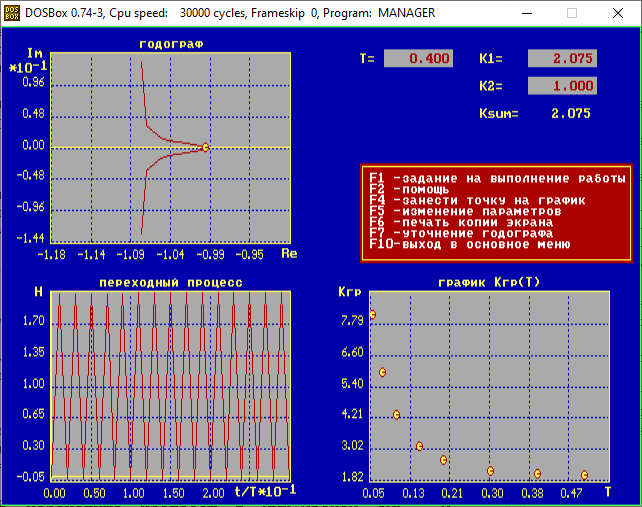
\includegraphics[width=\textwidth]{png/graph4.png}
			\centering{а)}
		\end{minipage} \begin{minipage}{.45\textwidth}
			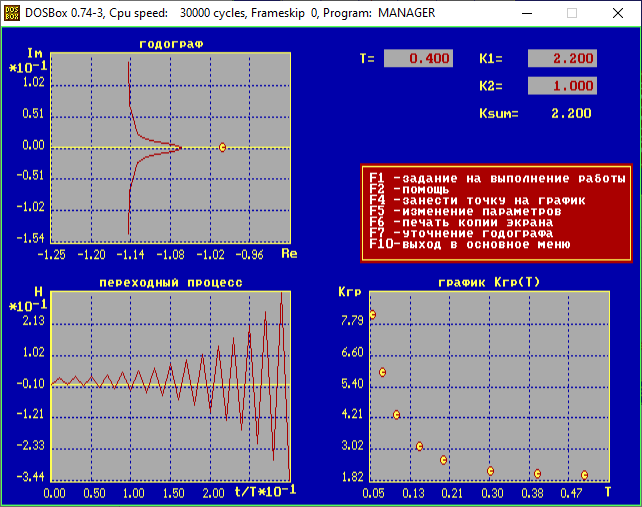
\includegraphics[width=\textwidth]{png/graph5.png}
			\centering{б)}
		\end{minipage}
		\begin{minipage}{.45\textwidth}
			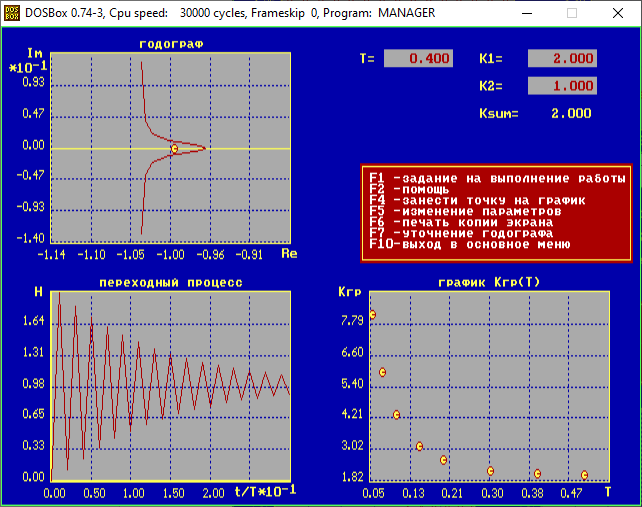
\includegraphics[width=\textwidth]{png/graph6.png}
			\centering{в)}
		\end{minipage} \begin{minipage}{.45\textwidth}
			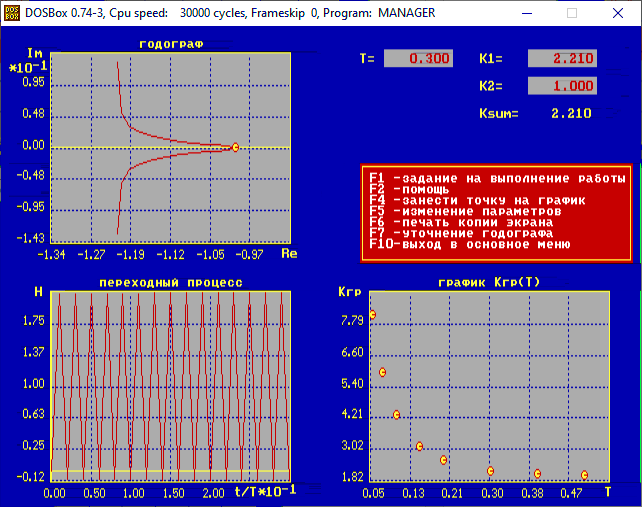
\includegraphics[width=\textwidth]{png/graph7.png}
			\centering{г)}
		\end{minipage}
		\captionof{figure}{Устойчивость замкнутой ИСАУ: а) нейтрально устойчива, б) неустойчива, в) устойчива, г) граница устойчивости для исходных параметров}
		\label{ustFig}
	\end{center}

	\section{Выводы}
	
	В данной работе была исследована возможность рассмотрения ИСАУ как САУ. Для недостаточно высоких частот квантования $\omega_0$ рассматриваемая ИСАУ значительно отличалась от соответствующей САУ. Но при уменьшении периода квантования $T$ или увеличении постоянной времени звена непрерывной части $T_1$ ИСАУ становилась более похожей на САУ (с точки зрения переходной функции), вплоть до отличия переходных процессов менее 10\%.
	
	Было исследовано влияние периода квантования на устойчивость ИСАУ. Имеется зависимость граничного коэффициента усиления $k_\text{гр}$ от периода квантования $T$, при чём нелинейная. В данном случае эта зависимость была получена аналитически, и она имеет вид $k_\text{гр} = 2\cth{\frac{T}{2T_1}}$.
	
\end{document}
